\documentclass[review,nonacm,screen,acmsmall,anonymous=true]{acmart}
\settopmatter{printfolios=false,printccs=false,printacmref=false}

\usepackage{listings,multirow,wrapfig,xspace,paralist}
\usepackage{xcolor,tikz,graphicx, pifont}
%\usetikzlibrary{positioning}

%% \newcommand{\authorcomment}[3]{\xspace\textcolor{#1}{{\bf #2} #3}\xspace}
\newcommand{\authorcomment}[3]{}


% For meta comments:
\newcommand{\isit}[1]{\authorcomment{cyan}{Check}{#1}}
\newcommand{\todo}[1]{\authorcomment{red}{TODO}{#1}}
\newcommand{\xmark}{\textcolor{red}{\ding{55}}}
\newcommand{\cmark}{\textcolor{green}{\ding{51}}}

\newcommand{\always}{\emph{Always}\xspace}
\newcommand{\sometimes}{\emph{Sometimes}\xspace}
\newcommand{\sometimesStar}{\emph{Sometimes*}\xspace}
\newcommand{\never}{\emph{Never}\xspace}
\newcommand{\neverStar}{\emph{Never*}\xspace}
\newcommand{\rdyn}{{\sf R-dyntrace}\xspace}
\newcommand{\instr}{{\sf InstrumentR}\xspace}

\definecolor{LightGray}{RGB}{247, 247, 247}
\definecolor{Gray}{rgb}{.3,.3,.3}
\definecolor{DarkGray}{rgb}{.5,.5,.5}

%% https://www.davehofmann.de/defining-custom-language-templates-for-latex-listings/
% Define Language
\lstdefinelanguage{smalleR} {
  % list of keywords
  morekeywords={
    for,
    if,
    else,
    function
  },
  sensitive=true, % keywords are not case-sensitive
  morecomment=[l]{\#}, % l is for line comment
  morestring=[b]{"} % defines that strings are enclosed in double quotes
}

\lstset{
  language={smalleR},
  columns=flexible,
  captionpos=b,
  frame=single,
  framerule=0pt,
  framexleftmargin=1mm,
  framexrightmargin=1mm,
  tabsize=2,
  belowskip=0pt,
  basicstyle=\small\ttfamily,
  backgroundcolor=\color{LightGray},
  emphstyle=\sffamily,
  keywordstyle=\bfseries,
  commentstyle=\color{Gray}\em,
  stringstyle=\color{Gray},
  alsoletter={., _, $},
  breaklines=true
}

\newcommand{\code}[1]{\lstinline |#1|\xspace}
\renewcommand{\c}[1]{\lstinline |#1|\xspace}
\newcommand{\strictr}{{\sf StrictR}\xspace}
\newcommand{\lazr}{{\sf LazR}\xspace}
\renewcommand{\Rsh}{{\sf\v R}\xspace}
\newcommand{\Rshstrict}{{\sf\v R-strict}\xspace}

\newcommand{\eg}{\emph{e.g.},\xspace}
\newcommand{\ie}{\emph{i.e.},\xspace}
\newcommand{\config}[1]{configuration \#{#1}}
\newcommand{\cconfig}[1]{Configuration \#{#1}}

\include{results}


\begin{document}


\begin{figure}[h]
  \centering
  % Created by tikzDevice version 0.12.3.1 on 2021-07-09 17:48:53
% !TEX encoding = UTF-8 Unicode
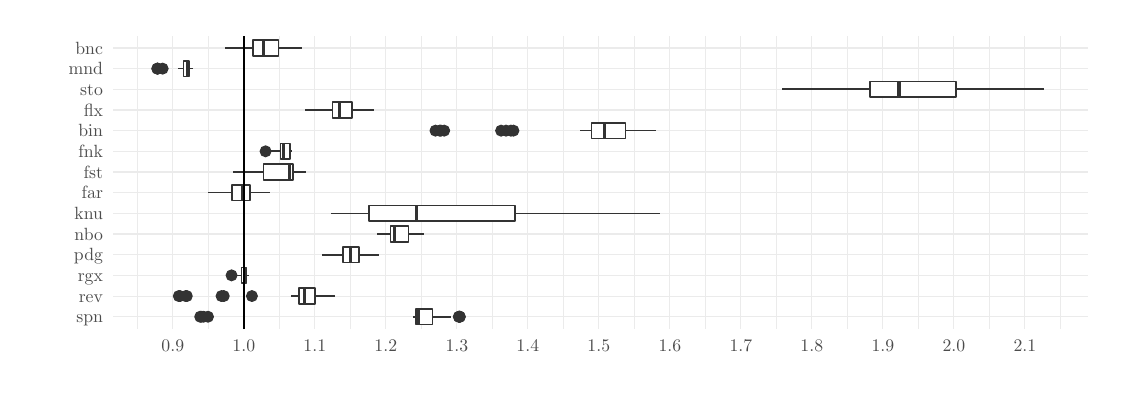
\begin{tikzpicture}[x=1pt,y=1pt]
\definecolor{fillColor}{RGB}{255,255,255}
\path[use as bounding box,fill=fillColor,fill opacity=0.00] (0,0) rectangle (390.26,130.09);
\begin{scope}
\path[clip] ( 30.80, 21.16) rectangle (383.14,127.24);
\definecolor{drawColor}{gray}{0.92}

\path[draw=drawColor,line width= 0.2pt,line join=round] ( 39.61, 21.16) --
	( 39.61,127.24);

\path[draw=drawColor,line width= 0.2pt,line join=round] ( 65.27, 21.16) --
	( 65.27,127.24);

\path[draw=drawColor,line width= 0.2pt,line join=round] ( 90.93, 21.16) --
	( 90.93,127.24);

\path[draw=drawColor,line width= 0.2pt,line join=round] (116.58, 21.16) --
	(116.58,127.24);

\path[draw=drawColor,line width= 0.2pt,line join=round] (142.24, 21.16) --
	(142.24,127.24);

\path[draw=drawColor,line width= 0.2pt,line join=round] (167.90, 21.16) --
	(167.90,127.24);

\path[draw=drawColor,line width= 0.2pt,line join=round] (193.55, 21.16) --
	(193.55,127.24);

\path[draw=drawColor,line width= 0.2pt,line join=round] (219.21, 21.16) --
	(219.21,127.24);

\path[draw=drawColor,line width= 0.2pt,line join=round] (244.87, 21.16) --
	(244.87,127.24);

\path[draw=drawColor,line width= 0.2pt,line join=round] (270.52, 21.16) --
	(270.52,127.24);

\path[draw=drawColor,line width= 0.2pt,line join=round] (296.18, 21.16) --
	(296.18,127.24);

\path[draw=drawColor,line width= 0.2pt,line join=round] (321.84, 21.16) --
	(321.84,127.24);

\path[draw=drawColor,line width= 0.2pt,line join=round] (347.50, 21.16) --
	(347.50,127.24);

\path[draw=drawColor,line width= 0.2pt,line join=round] (373.15, 21.16) --
	(373.15,127.24);

\path[draw=drawColor,line width= 0.4pt,line join=round] ( 30.80, 25.64) --
	(383.14, 25.64);

\path[draw=drawColor,line width= 0.4pt,line join=round] ( 30.80, 33.11) --
	(383.14, 33.11);

\path[draw=drawColor,line width= 0.4pt,line join=round] ( 30.80, 40.59) --
	(383.14, 40.59);

\path[draw=drawColor,line width= 0.4pt,line join=round] ( 30.80, 48.06) --
	(383.14, 48.06);

\path[draw=drawColor,line width= 0.4pt,line join=round] ( 30.80, 55.53) --
	(383.14, 55.53);

\path[draw=drawColor,line width= 0.4pt,line join=round] ( 30.80, 63.00) --
	(383.14, 63.00);

\path[draw=drawColor,line width= 0.4pt,line join=round] ( 30.80, 70.47) --
	(383.14, 70.47);

\path[draw=drawColor,line width= 0.4pt,line join=round] ( 30.80, 77.94) --
	(383.14, 77.94);

\path[draw=drawColor,line width= 0.4pt,line join=round] ( 30.80, 85.41) --
	(383.14, 85.41);

\path[draw=drawColor,line width= 0.4pt,line join=round] ( 30.80, 92.88) --
	(383.14, 92.88);

\path[draw=drawColor,line width= 0.4pt,line join=round] ( 30.80,100.35) --
	(383.14,100.35);

\path[draw=drawColor,line width= 0.4pt,line join=round] ( 30.80,107.82) --
	(383.14,107.82);

\path[draw=drawColor,line width= 0.4pt,line join=round] ( 30.80,115.29) --
	(383.14,115.29);

\path[draw=drawColor,line width= 0.4pt,line join=round] ( 30.80,122.76) --
	(383.14,122.76);

\path[draw=drawColor,line width= 0.4pt,line join=round] ( 52.44, 21.16) --
	( 52.44,127.24);

\path[draw=drawColor,line width= 0.4pt,line join=round] ( 78.10, 21.16) --
	( 78.10,127.24);

\path[draw=drawColor,line width= 0.4pt,line join=round] (103.75, 21.16) --
	(103.75,127.24);

\path[draw=drawColor,line width= 0.4pt,line join=round] (129.41, 21.16) --
	(129.41,127.24);

\path[draw=drawColor,line width= 0.4pt,line join=round] (155.07, 21.16) --
	(155.07,127.24);

\path[draw=drawColor,line width= 0.4pt,line join=round] (180.72, 21.16) --
	(180.72,127.24);

\path[draw=drawColor,line width= 0.4pt,line join=round] (206.38, 21.16) --
	(206.38,127.24);

\path[draw=drawColor,line width= 0.4pt,line join=round] (232.04, 21.16) --
	(232.04,127.24);

\path[draw=drawColor,line width= 0.4pt,line join=round] (257.70, 21.16) --
	(257.70,127.24);

\path[draw=drawColor,line width= 0.4pt,line join=round] (283.35, 21.16) --
	(283.35,127.24);

\path[draw=drawColor,line width= 0.4pt,line join=round] (309.01, 21.16) --
	(309.01,127.24);

\path[draw=drawColor,line width= 0.4pt,line join=round] (334.67, 21.16) --
	(334.67,127.24);

\path[draw=drawColor,line width= 0.4pt,line join=round] (360.32, 21.16) --
	(360.32,127.24);
\definecolor{drawColor}{gray}{0.20}
\definecolor{fillColor}{gray}{0.20}

\path[draw=drawColor,line width= 0.4pt,line join=round,line cap=round,fill=fillColor] (156.15, 25.64) circle (  1.96);

\path[draw=drawColor,line width= 0.4pt,line join=round,line cap=round,fill=fillColor] (156.12, 25.64) circle (  1.96);

\path[draw=drawColor,line width= 0.4pt,line join=round,line cap=round,fill=fillColor] (155.99, 25.64) circle (  1.96);

\path[draw=drawColor,line width= 0.4pt,line join=round,line cap=round,fill=fillColor] (155.93, 25.64) circle (  1.96);

\path[draw=drawColor,line width= 0.4pt,line join=round,line cap=round,fill=fillColor] (155.78, 25.64) circle (  1.96);

\path[draw=drawColor,line width= 0.4pt,line join=round,line cap=round,fill=fillColor] ( 65.16, 25.64) circle (  1.96);

\path[draw=drawColor,line width= 0.4pt,line join=round,line cap=round,fill=fillColor] ( 63.52, 25.64) circle (  1.96);

\path[draw=drawColor,line width= 0.4pt,line join=round,line cap=round,fill=fillColor] ( 62.73, 25.64) circle (  1.96);

\path[draw=drawColor,line width= 0.4pt,line join=round,line cap=round,fill=fillColor] ( 62.34, 25.64) circle (  1.96);

\path[draw=drawColor,line width= 0.6pt,line join=round] (146.25, 25.64) -- (152.79, 25.64);

\path[draw=drawColor,line width= 0.6pt,line join=round] (140.37, 25.64) -- (139.26, 25.64);
\definecolor{fillColor}{RGB}{255,255,255}

\path[draw=drawColor,line width= 0.6pt,line join=round,line cap=round,fill=fillColor] (146.25, 22.84) --
	(140.37, 22.84) --
	(140.37, 28.45) --
	(146.25, 28.45) --
	(146.25, 22.84) --
	cycle;

\path[draw=drawColor,line width= 1.1pt,line join=round] (141.25, 22.84) -- (141.25, 28.45);
\definecolor{fillColor}{gray}{0.20}

\path[draw=drawColor,line width= 0.4pt,line join=round,line cap=round,fill=fillColor] ( 81.03, 33.11) circle (  1.96);

\path[draw=drawColor,line width= 0.4pt,line join=round,line cap=round,fill=fillColor] ( 70.85, 33.11) circle (  1.96);

\path[draw=drawColor,line width= 0.4pt,line join=round,line cap=round,fill=fillColor] ( 70.05, 33.11) circle (  1.96);

\path[draw=drawColor,line width= 0.4pt,line join=round,line cap=round,fill=fillColor] ( 57.50, 33.11) circle (  1.96);

\path[draw=drawColor,line width= 0.4pt,line join=round,line cap=round,fill=fillColor] ( 57.11, 33.11) circle (  1.96);

\path[draw=drawColor,line width= 0.4pt,line join=round,line cap=round,fill=fillColor] ( 55.03, 33.11) circle (  1.96);

\path[draw=drawColor,line width= 0.4pt,line join=round,line cap=round,fill=fillColor] ( 54.61, 33.11) circle (  1.96);

\path[draw=drawColor,line width= 0.6pt,line join=round] (103.83, 33.11) -- (110.91, 33.11);

\path[draw=drawColor,line width= 0.6pt,line join=round] ( 98.16, 33.11) -- ( 95.23, 33.11);
\definecolor{fillColor}{RGB}{255,255,255}

\path[draw=drawColor,line width= 0.6pt,line join=round,line cap=round,fill=fillColor] (103.83, 30.31) --
	( 98.16, 30.31) --
	( 98.16, 35.92) --
	(103.83, 35.92) --
	(103.83, 30.31) --
	cycle;

\path[draw=drawColor,line width= 1.1pt,line join=round] (100.11, 30.31) -- (100.11, 35.92);
\definecolor{fillColor}{gray}{0.20}

\path[draw=drawColor,line width= 0.4pt,line join=round,line cap=round,fill=fillColor] ( 73.67, 40.59) circle (  1.96);

\path[draw=drawColor,line width= 0.6pt,line join=round] ( 79.10, 40.59) -- ( 79.80, 40.59);

\path[draw=drawColor,line width= 0.6pt,line join=round] ( 77.25, 40.59) -- ( 74.95, 40.59);
\definecolor{fillColor}{RGB}{255,255,255}

\path[draw=drawColor,line width= 0.6pt,line join=round,line cap=round,fill=fillColor] ( 79.10, 37.78) --
	( 77.25, 37.78) --
	( 77.25, 43.39) --
	( 79.10, 43.39) --
	( 79.10, 37.78) --
	cycle;

\path[draw=drawColor,line width= 1.1pt,line join=round] ( 78.68, 37.78) -- ( 78.68, 43.39);

\path[draw=drawColor,line width= 0.6pt,line join=round] (119.62, 48.06) -- (126.98, 48.06);

\path[draw=drawColor,line width= 0.6pt,line join=round] (113.92, 48.06) -- (106.44, 48.06);

\path[draw=drawColor,line width= 0.6pt,line join=round,line cap=round,fill=fillColor] (119.62, 45.25) --
	(113.92, 45.25) --
	(113.92, 50.86) --
	(119.62, 50.86) --
	(119.62, 45.25) --
	cycle;

\path[draw=drawColor,line width= 1.1pt,line join=round] (116.71, 45.25) -- (116.71, 50.86);

\path[draw=drawColor,line width= 0.6pt,line join=round] (137.64, 55.53) -- (143.32, 55.53);

\path[draw=drawColor,line width= 0.6pt,line join=round] (131.11, 55.53) -- (126.10, 55.53);

\path[draw=drawColor,line width= 0.6pt,line join=round,line cap=round,fill=fillColor] (137.64, 52.72) --
	(131.11, 52.72) --
	(131.11, 58.33) --
	(137.64, 58.33) --
	(137.64, 52.72) --
	cycle;

\path[draw=drawColor,line width= 1.1pt,line join=round] (132.52, 52.72) -- (132.52, 58.33);

\path[draw=drawColor,line width= 0.6pt,line join=round] (176.13, 63.00) -- (228.50, 63.00);

\path[draw=drawColor,line width= 0.6pt,line join=round] (123.24, 63.00) -- (109.43, 63.00);

\path[draw=drawColor,line width= 0.6pt,line join=round,line cap=round,fill=fillColor] (176.13, 60.19) --
	(123.24, 60.19) --
	(123.24, 65.80) --
	(176.13, 65.80) --
	(176.13, 60.19) --
	cycle;

\path[draw=drawColor,line width= 1.1pt,line join=round] (140.40, 60.19) -- (140.40, 65.80);

\path[draw=drawColor,line width= 0.6pt,line join=round] ( 80.43, 70.47) -- ( 87.42, 70.47);

\path[draw=drawColor,line width= 0.6pt,line join=round] ( 73.78, 70.47) -- ( 65.12, 70.47);

\path[draw=drawColor,line width= 0.6pt,line join=round,line cap=round,fill=fillColor] ( 80.43, 67.66) --
	( 73.78, 67.66) --
	( 73.78, 73.27) --
	( 80.43, 73.27) --
	( 80.43, 67.66) --
	cycle;

\path[draw=drawColor,line width= 1.1pt,line join=round] ( 77.51, 67.66) -- ( 77.51, 73.27);

\path[draw=drawColor,line width= 0.6pt,line join=round] ( 95.85, 77.94) -- (100.61, 77.94);

\path[draw=drawColor,line width= 0.6pt,line join=round] ( 85.22, 77.94) -- ( 74.17, 77.94);

\path[draw=drawColor,line width= 0.6pt,line join=round,line cap=round,fill=fillColor] ( 95.85, 75.14) --
	( 85.22, 75.14) --
	( 85.22, 80.74) --
	( 95.85, 80.74) --
	( 95.85, 75.14) --
	cycle;

\path[draw=drawColor,line width= 1.1pt,line join=round] ( 94.47, 75.14) -- ( 94.47, 80.74);
\definecolor{fillColor}{gray}{0.20}

\path[draw=drawColor,line width= 0.4pt,line join=round,line cap=round,fill=fillColor] ( 85.96, 85.41) circle (  1.96);

\path[draw=drawColor,line width= 0.6pt,line join=round] ( 94.71, 85.41) -- ( 95.48, 85.41);

\path[draw=drawColor,line width= 0.6pt,line join=round] ( 91.33, 85.41) -- ( 87.02, 85.41);
\definecolor{fillColor}{RGB}{255,255,255}

\path[draw=drawColor,line width= 0.6pt,line join=round,line cap=round,fill=fillColor] ( 94.71, 82.61) --
	( 91.33, 82.61) --
	( 91.33, 88.21) --
	( 94.71, 88.21) --
	( 94.71, 82.61) --
	cycle;

\path[draw=drawColor,line width= 1.1pt,line join=round] ( 92.53, 82.61) -- ( 92.53, 88.21);
\definecolor{fillColor}{gray}{0.20}

\path[draw=drawColor,line width= 0.4pt,line join=round,line cap=round,fill=fillColor] (175.53, 92.88) circle (  1.96);

\path[draw=drawColor,line width= 0.4pt,line join=round,line cap=round,fill=fillColor] (174.60, 92.88) circle (  1.96);

\path[draw=drawColor,line width= 0.4pt,line join=round,line cap=round,fill=fillColor] (172.86, 92.88) circle (  1.96);

\path[draw=drawColor,line width= 0.4pt,line join=round,line cap=round,fill=fillColor] (171.07, 92.88) circle (  1.96);

\path[draw=drawColor,line width= 0.4pt,line join=round,line cap=round,fill=fillColor] (150.51, 92.88) circle (  1.96);

\path[draw=drawColor,line width= 0.4pt,line join=round,line cap=round,fill=fillColor] (149.30, 92.88) circle (  1.96);

\path[draw=drawColor,line width= 0.4pt,line join=round,line cap=round,fill=fillColor] (148.89, 92.88) circle (  1.96);

\path[draw=drawColor,line width= 0.4pt,line join=round,line cap=round,fill=fillColor] (147.36, 92.88) circle (  1.96);

\path[draw=drawColor,line width= 0.6pt,line join=round] (215.97, 92.88) -- (227.06, 92.88);

\path[draw=drawColor,line width= 0.6pt,line join=round] (203.77, 92.88) -- (199.42, 92.88);
\definecolor{fillColor}{RGB}{255,255,255}

\path[draw=drawColor,line width= 0.6pt,line join=round,line cap=round,fill=fillColor] (215.97, 90.08) --
	(203.77, 90.08) --
	(203.77, 95.68) --
	(215.97, 95.68) --
	(215.97, 90.08) --
	cycle;

\path[draw=drawColor,line width= 1.1pt,line join=round] (208.57, 90.08) -- (208.57, 95.68);

\path[draw=drawColor,line width= 0.6pt,line join=round] (117.23,100.35) -- (125.27,100.35);

\path[draw=drawColor,line width= 0.6pt,line join=round] (110.12,100.35) -- (100.09,100.35);

\path[draw=drawColor,line width= 0.6pt,line join=round,line cap=round,fill=fillColor] (117.23, 97.55) --
	(110.12, 97.55) --
	(110.12,103.15) --
	(117.23,103.15) --
	(117.23, 97.55) --
	cycle;

\path[draw=drawColor,line width= 1.1pt,line join=round] (112.68, 97.55) -- (112.68,103.15);

\path[draw=drawColor,line width= 0.6pt,line join=round] (335.48,107.82) -- (367.13,107.82);

\path[draw=drawColor,line width= 0.6pt,line join=round] (304.34,107.82) -- (272.46,107.82);

\path[draw=drawColor,line width= 0.6pt,line join=round,line cap=round,fill=fillColor] (335.48,105.02) --
	(304.34,105.02) --
	(304.34,110.62) --
	(335.48,110.62) --
	(335.48,105.02) --
	cycle;

\path[draw=drawColor,line width= 1.1pt,line join=round] (314.85,105.02) -- (314.85,110.62);
\definecolor{fillColor}{gray}{0.20}

\path[draw=drawColor,line width= 0.4pt,line join=round,line cap=round,fill=fillColor] ( 48.77,115.29) circle (  1.96);

\path[draw=drawColor,line width= 0.4pt,line join=round,line cap=round,fill=fillColor] ( 47.00,115.29) circle (  1.96);

\path[draw=drawColor,line width= 0.4pt,line join=round,line cap=round,fill=fillColor] ( 46.92,115.29) circle (  1.96);

\path[draw=drawColor,line width= 0.4pt,line join=round,line cap=round,fill=fillColor] ( 46.81,115.29) circle (  1.96);

\path[draw=drawColor,line width= 0.6pt,line join=round] ( 58.27,115.29) -- ( 59.68,115.29);

\path[draw=drawColor,line width= 0.6pt,line join=round] ( 56.36,115.29) -- ( 54.49,115.29);
\definecolor{fillColor}{RGB}{255,255,255}

\path[draw=drawColor,line width= 0.6pt,line join=round,line cap=round,fill=fillColor] ( 58.27,112.49) --
	( 56.36,112.49) --
	( 56.36,118.09) --
	( 58.27,118.09) --
	( 58.27,112.49) --
	cycle;

\path[draw=drawColor,line width= 1.1pt,line join=round] ( 57.71,112.49) -- ( 57.71,118.09);

\path[draw=drawColor,line width= 0.6pt,line join=round] ( 90.59,122.76) -- ( 99.03,122.76);

\path[draw=drawColor,line width= 0.6pt,line join=round] ( 81.46,122.76) -- ( 71.38,122.76);

\path[draw=drawColor,line width= 0.6pt,line join=round,line cap=round,fill=fillColor] ( 90.59,119.96) --
	( 81.46,119.96) --
	( 81.46,125.56) --
	( 90.59,125.56) --
	( 90.59,119.96) --
	cycle;

\path[draw=drawColor,line width= 1.1pt,line join=round] ( 85.21,119.96) -- ( 85.21,125.56);
\definecolor{drawColor}{RGB}{0,0,0}

\path[draw=drawColor,line width= 0.6pt,line join=round] ( 78.10, 21.16) -- ( 78.10,127.24);
\end{scope}
\begin{scope}
\path[clip] (  0.00,  0.00) rectangle (390.26,130.09);
\definecolor{drawColor}{gray}{0.30}

\node[text=drawColor,anchor=base east,inner sep=0pt, outer sep=0pt, scale=  0.64] at ( 27.20, 23.44) {spn};

\node[text=drawColor,anchor=base east,inner sep=0pt, outer sep=0pt, scale=  0.64] at ( 27.20, 30.91) {rev};

\node[text=drawColor,anchor=base east,inner sep=0pt, outer sep=0pt, scale=  0.64] at ( 27.20, 38.38) {rgx};

\node[text=drawColor,anchor=base east,inner sep=0pt, outer sep=0pt, scale=  0.64] at ( 27.20, 45.85) {pdg};

\node[text=drawColor,anchor=base east,inner sep=0pt, outer sep=0pt, scale=  0.64] at ( 27.20, 53.32) {nbo};

\node[text=drawColor,anchor=base east,inner sep=0pt, outer sep=0pt, scale=  0.64] at ( 27.20, 60.79) {knu};

\node[text=drawColor,anchor=base east,inner sep=0pt, outer sep=0pt, scale=  0.64] at ( 27.20, 68.26) {far};

\node[text=drawColor,anchor=base east,inner sep=0pt, outer sep=0pt, scale=  0.64] at ( 27.20, 75.73) {fst};

\node[text=drawColor,anchor=base east,inner sep=0pt, outer sep=0pt, scale=  0.64] at ( 27.20, 83.20) {fnk};

\node[text=drawColor,anchor=base east,inner sep=0pt, outer sep=0pt, scale=  0.64] at ( 27.20, 90.67) {bin};

\node[text=drawColor,anchor=base east,inner sep=0pt, outer sep=0pt, scale=  0.64] at ( 27.20, 98.14) {flx};

\node[text=drawColor,anchor=base east,inner sep=0pt, outer sep=0pt, scale=  0.64] at ( 27.20,105.61) {sto};

\node[text=drawColor,anchor=base east,inner sep=0pt, outer sep=0pt, scale=  0.64] at ( 27.20,113.08) {mnd};

\node[text=drawColor,anchor=base east,inner sep=0pt, outer sep=0pt, scale=  0.64] at ( 27.20,120.55) {bnc};
\end{scope}
\begin{scope}
\path[clip] (  0.00,  0.00) rectangle (390.26,130.09);
\definecolor{drawColor}{gray}{0.30}

\node[text=drawColor,anchor=base,inner sep=0pt, outer sep=0pt, scale=  0.64] at ( 52.44, 13.15) {0.9};

\node[text=drawColor,anchor=base,inner sep=0pt, outer sep=0pt, scale=  0.64] at ( 78.10, 13.15) {1.0};

\node[text=drawColor,anchor=base,inner sep=0pt, outer sep=0pt, scale=  0.64] at (103.75, 13.15) {1.1};

\node[text=drawColor,anchor=base,inner sep=0pt, outer sep=0pt, scale=  0.64] at (129.41, 13.15) {1.2};

\node[text=drawColor,anchor=base,inner sep=0pt, outer sep=0pt, scale=  0.64] at (155.07, 13.15) {1.3};

\node[text=drawColor,anchor=base,inner sep=0pt, outer sep=0pt, scale=  0.64] at (180.72, 13.15) {1.4};

\node[text=drawColor,anchor=base,inner sep=0pt, outer sep=0pt, scale=  0.64] at (206.38, 13.15) {1.5};

\node[text=drawColor,anchor=base,inner sep=0pt, outer sep=0pt, scale=  0.64] at (232.04, 13.15) {1.6};

\node[text=drawColor,anchor=base,inner sep=0pt, outer sep=0pt, scale=  0.64] at (257.70, 13.15) {1.7};

\node[text=drawColor,anchor=base,inner sep=0pt, outer sep=0pt, scale=  0.64] at (283.35, 13.15) {1.8};

\node[text=drawColor,anchor=base,inner sep=0pt, outer sep=0pt, scale=  0.64] at (309.01, 13.15) {1.9};

\node[text=drawColor,anchor=base,inner sep=0pt, outer sep=0pt, scale=  0.64] at (334.67, 13.15) {2.0};

\node[text=drawColor,anchor=base,inner sep=0pt, outer sep=0pt, scale=  0.64] at (360.32, 13.15) {2.1};
\end{scope}
\end{tikzpicture}

  \caption{Speedup of \Rshstrict}
  \label{fig:speedup}
\end{figure}

\begin{figure}[h]
  \centering
  % Created by tikzDevice version 0.12.3.1 on 2021-07-08 14:51:17
% !TEX encoding = UTF-8 Unicode
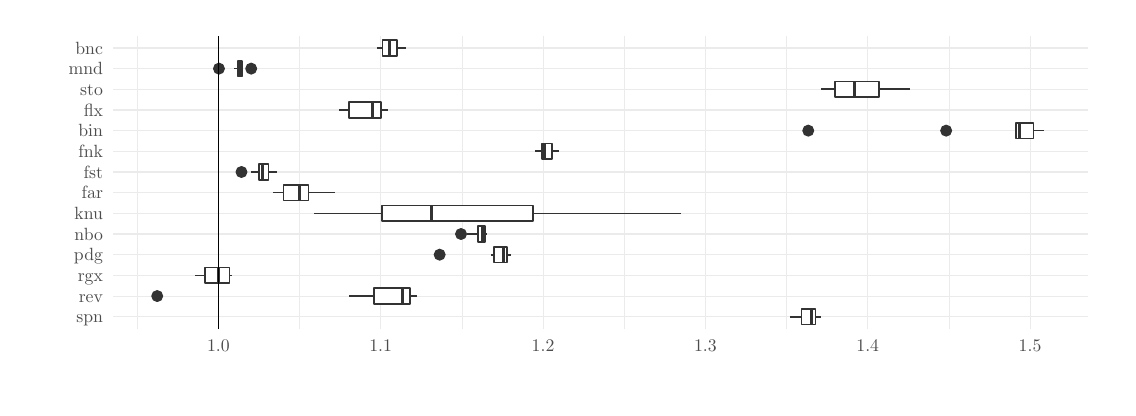
\begin{tikzpicture}[x=1pt,y=1pt]
\definecolor{fillColor}{RGB}{255,255,255}
\path[use as bounding box,fill=fillColor,fill opacity=0.00] (0,0) rectangle (390.26,130.09);
\begin{scope}
\path[clip] ( 30.80, 21.16) rectangle (383.14,127.24);
\definecolor{drawColor}{gray}{0.92}

\path[draw=drawColor,line width= 0.2pt,line join=round] ( 39.57, 21.16) --
	( 39.57,127.24);

\path[draw=drawColor,line width= 0.2pt,line join=round] ( 98.23, 21.16) --
	( 98.23,127.24);

\path[draw=drawColor,line width= 0.2pt,line join=round] (156.90, 21.16) --
	(156.90,127.24);

\path[draw=drawColor,line width= 0.2pt,line join=round] (215.56, 21.16) --
	(215.56,127.24);

\path[draw=drawColor,line width= 0.2pt,line join=round] (274.22, 21.16) --
	(274.22,127.24);

\path[draw=drawColor,line width= 0.2pt,line join=round] (332.88, 21.16) --
	(332.88,127.24);

\path[draw=drawColor,line width= 0.4pt,line join=round] ( 30.80, 25.64) --
	(383.14, 25.64);

\path[draw=drawColor,line width= 0.4pt,line join=round] ( 30.80, 33.11) --
	(383.14, 33.11);

\path[draw=drawColor,line width= 0.4pt,line join=round] ( 30.80, 40.59) --
	(383.14, 40.59);

\path[draw=drawColor,line width= 0.4pt,line join=round] ( 30.80, 48.06) --
	(383.14, 48.06);

\path[draw=drawColor,line width= 0.4pt,line join=round] ( 30.80, 55.53) --
	(383.14, 55.53);

\path[draw=drawColor,line width= 0.4pt,line join=round] ( 30.80, 63.00) --
	(383.14, 63.00);

\path[draw=drawColor,line width= 0.4pt,line join=round] ( 30.80, 70.47) --
	(383.14, 70.47);

\path[draw=drawColor,line width= 0.4pt,line join=round] ( 30.80, 77.94) --
	(383.14, 77.94);

\path[draw=drawColor,line width= 0.4pt,line join=round] ( 30.80, 85.41) --
	(383.14, 85.41);

\path[draw=drawColor,line width= 0.4pt,line join=round] ( 30.80, 92.88) --
	(383.14, 92.88);

\path[draw=drawColor,line width= 0.4pt,line join=round] ( 30.80,100.35) --
	(383.14,100.35);

\path[draw=drawColor,line width= 0.4pt,line join=round] ( 30.80,107.82) --
	(383.14,107.82);

\path[draw=drawColor,line width= 0.4pt,line join=round] ( 30.80,115.29) --
	(383.14,115.29);

\path[draw=drawColor,line width= 0.4pt,line join=round] ( 30.80,122.76) --
	(383.14,122.76);

\path[draw=drawColor,line width= 0.4pt,line join=round] ( 68.90, 21.16) --
	( 68.90,127.24);

\path[draw=drawColor,line width= 0.4pt,line join=round] (127.56, 21.16) --
	(127.56,127.24);

\path[draw=drawColor,line width= 0.4pt,line join=round] (186.23, 21.16) --
	(186.23,127.24);

\path[draw=drawColor,line width= 0.4pt,line join=round] (244.89, 21.16) --
	(244.89,127.24);

\path[draw=drawColor,line width= 0.4pt,line join=round] (303.55, 21.16) --
	(303.55,127.24);

\path[draw=drawColor,line width= 0.4pt,line join=round] (362.21, 21.16) --
	(362.21,127.24);
\definecolor{drawColor}{gray}{0.20}

\path[draw=drawColor,line width= 0.6pt,line join=round] (284.63, 25.64) -- (286.77, 25.64);

\path[draw=drawColor,line width= 0.6pt,line join=round] (279.56, 25.64) -- (275.43, 25.64);
\definecolor{fillColor}{RGB}{255,255,255}

\path[draw=drawColor,line width= 0.6pt,line join=round,line cap=round,fill=fillColor] (284.63, 22.84) --
	(279.56, 22.84) --
	(279.56, 28.45) --
	(284.63, 28.45) --
	(284.63, 22.84) --
	cycle;

\path[draw=drawColor,line width= 1.1pt,line join=round] (283.24, 22.84) -- (283.24, 28.45);
\definecolor{fillColor}{gray}{0.20}

\path[draw=drawColor,line width= 0.4pt,line join=round,line cap=round,fill=fillColor] ( 46.81, 33.11) circle (  1.96);

\path[draw=drawColor,line width= 0.6pt,line join=round] (138.05, 33.11) -- (140.85, 33.11);

\path[draw=drawColor,line width= 0.6pt,line join=round] (125.16, 33.11) -- (116.17, 33.11);
\definecolor{fillColor}{RGB}{255,255,255}

\path[draw=drawColor,line width= 0.6pt,line join=round,line cap=round,fill=fillColor] (138.05, 30.31) --
	(125.16, 30.31) --
	(125.16, 35.92) --
	(138.05, 35.92) --
	(138.05, 30.31) --
	cycle;

\path[draw=drawColor,line width= 1.1pt,line join=round] (135.47, 30.31) -- (135.47, 35.92);

\path[draw=drawColor,line width= 0.6pt,line join=round] ( 72.98, 40.59) -- ( 73.85, 40.59);

\path[draw=drawColor,line width= 0.6pt,line join=round] ( 64.12, 40.59) -- ( 60.29, 40.59);

\path[draw=drawColor,line width= 0.6pt,line join=round,line cap=round,fill=fillColor] ( 72.98, 37.78) --
	( 64.12, 37.78) --
	( 64.12, 43.39) --
	( 72.98, 43.39) --
	( 72.98, 37.78) --
	cycle;

\path[draw=drawColor,line width= 1.1pt,line join=round] ( 68.80, 37.78) -- ( 68.80, 43.39);
\definecolor{fillColor}{gray}{0.20}

\path[draw=drawColor,line width= 0.4pt,line join=round,line cap=round,fill=fillColor] (148.87, 48.06) circle (  1.96);

\path[draw=drawColor,line width= 0.6pt,line join=round] (173.09, 48.06) -- (174.57, 48.06);

\path[draw=drawColor,line width= 0.6pt,line join=round] (168.54, 48.06) -- (167.60, 48.06);
\definecolor{fillColor}{RGB}{255,255,255}

\path[draw=drawColor,line width= 0.6pt,line join=round,line cap=round,fill=fillColor] (173.09, 45.25) --
	(168.54, 45.25) --
	(168.54, 50.86) --
	(173.09, 50.86) --
	(173.09, 45.25) --
	cycle;

\path[draw=drawColor,line width= 1.1pt,line join=round] (172.07, 45.25) -- (172.07, 50.86);
\definecolor{fillColor}{gray}{0.20}

\path[draw=drawColor,line width= 0.4pt,line join=round,line cap=round,fill=fillColor] (156.59, 55.53) circle (  1.96);

\path[draw=drawColor,line width= 0.6pt,line join=round] (165.34, 55.53) -- (166.01, 55.53);

\path[draw=drawColor,line width= 0.6pt,line join=round] (162.66, 55.53) -- (158.81, 55.53);
\definecolor{fillColor}{RGB}{255,255,255}

\path[draw=drawColor,line width= 0.6pt,line join=round,line cap=round,fill=fillColor] (165.34, 52.72) --
	(162.66, 52.72) --
	(162.66, 58.33) --
	(165.34, 58.33) --
	(165.34, 52.72) --
	cycle;

\path[draw=drawColor,line width= 1.1pt,line join=round] (164.48, 52.72) -- (164.48, 58.33);

\path[draw=drawColor,line width= 0.6pt,line join=round] (182.58, 63.00) -- (235.90, 63.00);

\path[draw=drawColor,line width= 0.6pt,line join=round] (128.01, 63.00) -- (103.32, 63.00);

\path[draw=drawColor,line width= 0.6pt,line join=round,line cap=round,fill=fillColor] (182.58, 60.19) --
	(128.01, 60.19) --
	(128.01, 65.80) --
	(182.58, 65.80) --
	(182.58, 60.19) --
	cycle;

\path[draw=drawColor,line width= 1.1pt,line join=round] (145.89, 60.19) -- (145.89, 65.80);

\path[draw=drawColor,line width= 0.6pt,line join=round] (101.45, 70.47) -- (110.90, 70.47);

\path[draw=drawColor,line width= 0.6pt,line join=round] ( 92.47, 70.47) -- ( 88.47, 70.47);

\path[draw=drawColor,line width= 0.6pt,line join=round,line cap=round,fill=fillColor] (101.45, 67.66) --
	( 92.47, 67.66) --
	( 92.47, 73.27) --
	(101.45, 73.27) --
	(101.45, 67.66) --
	cycle;

\path[draw=drawColor,line width= 1.1pt,line join=round] ( 98.22, 67.66) -- ( 98.22, 73.27);
\definecolor{fillColor}{gray}{0.20}

\path[draw=drawColor,line width= 0.4pt,line join=round,line cap=round,fill=fillColor] ( 77.26, 77.94) circle (  1.96);

\path[draw=drawColor,line width= 0.6pt,line join=round] ( 87.06, 77.94) -- ( 90.24, 77.94);

\path[draw=drawColor,line width= 0.6pt,line join=round] ( 83.61, 77.94) -- ( 80.73, 77.94);
\definecolor{fillColor}{RGB}{255,255,255}

\path[draw=drawColor,line width= 0.6pt,line join=round,line cap=round,fill=fillColor] ( 87.06, 75.14) --
	( 83.61, 75.14) --
	( 83.61, 80.74) --
	( 87.06, 80.74) --
	( 87.06, 75.14) --
	cycle;

\path[draw=drawColor,line width= 1.1pt,line join=round] ( 84.91, 75.14) -- ( 84.91, 80.74);

\path[draw=drawColor,line width= 0.6pt,line join=round] (189.41, 85.41) -- (192.04, 85.41);

\path[draw=drawColor,line width= 0.6pt,line join=round] (185.92, 85.41) -- (183.50, 85.41);

\path[draw=drawColor,line width= 0.6pt,line join=round,line cap=round,fill=fillColor] (189.41, 82.61) --
	(185.92, 82.61) --
	(185.92, 88.21) --
	(189.41, 88.21) --
	(189.41, 82.61) --
	cycle;

\path[draw=drawColor,line width= 1.1pt,line join=round] (186.70, 82.61) -- (186.70, 88.21);
\definecolor{fillColor}{gray}{0.20}

\path[draw=drawColor,line width= 0.4pt,line join=round,line cap=round,fill=fillColor] (331.89, 92.88) circle (  1.96);

\path[draw=drawColor,line width= 0.4pt,line join=round,line cap=round,fill=fillColor] (282.06, 92.88) circle (  1.96);

\path[draw=drawColor,line width= 0.6pt,line join=round] (363.43, 92.88) -- (367.13, 92.88);

\path[draw=drawColor,line width= 0.6pt,line join=round] (357.10, 92.88) -- (356.92, 92.88);
\definecolor{fillColor}{RGB}{255,255,255}

\path[draw=drawColor,line width= 0.6pt,line join=round,line cap=round,fill=fillColor] (363.43, 90.08) --
	(357.10, 90.08) --
	(357.10, 95.68) --
	(363.43, 95.68) --
	(363.43, 90.08) --
	cycle;

\path[draw=drawColor,line width= 1.1pt,line join=round] (358.53, 90.08) -- (358.53, 95.68);

\path[draw=drawColor,line width= 0.6pt,line join=round] (127.74,100.35) -- (130.23,100.35);

\path[draw=drawColor,line width= 0.6pt,line join=round] (116.20,100.35) -- (112.36,100.35);

\path[draw=drawColor,line width= 0.6pt,line join=round,line cap=round,fill=fillColor] (127.74, 97.55) --
	(116.20, 97.55) --
	(116.20,103.15) --
	(127.74,103.15) --
	(127.74, 97.55) --
	cycle;

\path[draw=drawColor,line width= 1.1pt,line join=round] (124.62, 97.55) -- (124.62,103.15);

\path[draw=drawColor,line width= 0.6pt,line join=round] (307.66,107.82) -- (318.79,107.82);

\path[draw=drawColor,line width= 0.6pt,line join=round] (291.62,107.82) -- (286.82,107.82);

\path[draw=drawColor,line width= 0.6pt,line join=round,line cap=round,fill=fillColor] (307.66,105.02) --
	(291.62,105.02) --
	(291.62,110.62) --
	(307.66,110.62) --
	(307.66,105.02) --
	cycle;

\path[draw=drawColor,line width= 1.1pt,line join=round] (298.63,105.02) -- (298.63,110.62);
\definecolor{fillColor}{gray}{0.20}

\path[draw=drawColor,line width= 0.4pt,line join=round,line cap=round,fill=fillColor] ( 80.77,115.29) circle (  1.96);

\path[draw=drawColor,line width= 0.4pt,line join=round,line cap=round,fill=fillColor] ( 69.12,115.29) circle (  1.96);

\path[draw=drawColor,line width= 0.6pt,line join=round] ( 77.54,115.29) -- ( 77.81,115.29);

\path[draw=drawColor,line width= 0.6pt,line join=round] ( 76.09,115.29) -- ( 74.46,115.29);
\definecolor{fillColor}{RGB}{255,255,255}

\path[draw=drawColor,line width= 0.6pt,line join=round,line cap=round,fill=fillColor] ( 77.54,112.49) --
	( 76.09,112.49) --
	( 76.09,118.09) --
	( 77.54,118.09) --
	( 77.54,112.49) --
	cycle;

\path[draw=drawColor,line width= 1.1pt,line join=round] ( 76.62,112.49) -- ( 76.62,118.09);

\path[draw=drawColor,line width= 0.6pt,line join=round] (133.55,122.76) -- (136.80,122.76);

\path[draw=drawColor,line width= 0.6pt,line join=round] (128.16,122.76) -- (126.25,122.76);

\path[draw=drawColor,line width= 0.6pt,line join=round,line cap=round,fill=fillColor] (133.55,119.96) --
	(128.16,119.96) --
	(128.16,125.56) --
	(133.55,125.56) --
	(133.55,119.96) --
	cycle;

\path[draw=drawColor,line width= 1.1pt,line join=round] (130.87,119.96) -- (130.87,125.56);
\definecolor{drawColor}{RGB}{0,0,0}

\path[draw=drawColor,line width= 0.6pt,line join=round] ( 68.90, 21.16) -- ( 68.90,127.24);
\end{scope}
\begin{scope}
\path[clip] (  0.00,  0.00) rectangle (390.26,130.09);
\definecolor{drawColor}{gray}{0.30}

\node[text=drawColor,anchor=base east,inner sep=0pt, outer sep=0pt, scale=  0.64] at ( 27.20, 23.44) {spn};

\node[text=drawColor,anchor=base east,inner sep=0pt, outer sep=0pt, scale=  0.64] at ( 27.20, 30.91) {rev};

\node[text=drawColor,anchor=base east,inner sep=0pt, outer sep=0pt, scale=  0.64] at ( 27.20, 38.38) {rgx};

\node[text=drawColor,anchor=base east,inner sep=0pt, outer sep=0pt, scale=  0.64] at ( 27.20, 45.85) {pdg};

\node[text=drawColor,anchor=base east,inner sep=0pt, outer sep=0pt, scale=  0.64] at ( 27.20, 53.32) {nbo};

\node[text=drawColor,anchor=base east,inner sep=0pt, outer sep=0pt, scale=  0.64] at ( 27.20, 60.79) {knu};

\node[text=drawColor,anchor=base east,inner sep=0pt, outer sep=0pt, scale=  0.64] at ( 27.20, 68.26) {far};

\node[text=drawColor,anchor=base east,inner sep=0pt, outer sep=0pt, scale=  0.64] at ( 27.20, 75.73) {fst};

\node[text=drawColor,anchor=base east,inner sep=0pt, outer sep=0pt, scale=  0.64] at ( 27.20, 83.20) {fnk};

\node[text=drawColor,anchor=base east,inner sep=0pt, outer sep=0pt, scale=  0.64] at ( 27.20, 90.67) {bin};

\node[text=drawColor,anchor=base east,inner sep=0pt, outer sep=0pt, scale=  0.64] at ( 27.20, 98.14) {flx};

\node[text=drawColor,anchor=base east,inner sep=0pt, outer sep=0pt, scale=  0.64] at ( 27.20,105.61) {sto};

\node[text=drawColor,anchor=base east,inner sep=0pt, outer sep=0pt, scale=  0.64] at ( 27.20,113.08) {mnd};

\node[text=drawColor,anchor=base east,inner sep=0pt, outer sep=0pt, scale=  0.64] at ( 27.20,120.55) {bnc};
\end{scope}
\begin{scope}
\path[clip] (  0.00,  0.00) rectangle (390.26,130.09);
\definecolor{drawColor}{gray}{0.30}

\node[text=drawColor,anchor=base,inner sep=0pt, outer sep=0pt, scale=  0.64] at ( 68.90, 13.15) {1.0};

\node[text=drawColor,anchor=base,inner sep=0pt, outer sep=0pt, scale=  0.64] at (127.56, 13.15) {1.1};

\node[text=drawColor,anchor=base,inner sep=0pt, outer sep=0pt, scale=  0.64] at (186.23, 13.15) {1.2};

\node[text=drawColor,anchor=base,inner sep=0pt, outer sep=0pt, scale=  0.64] at (244.89, 13.15) {1.3};

\node[text=drawColor,anchor=base,inner sep=0pt, outer sep=0pt, scale=  0.64] at (303.55, 13.15) {1.4};

\node[text=drawColor,anchor=base,inner sep=0pt, outer sep=0pt, scale=  0.64] at (362.21, 13.15) {1.5};
\end{scope}
\end{tikzpicture}

  \caption{Speedup of \Rshstrict without optimizations}
  \label{fig:speedup-bc}
\end{figure}

% \begin{figure}[h]
%   \centering
%   % Created by tikzDevice version 0.12.3.1 on 2021-07-09 17:48:57
% !TEX encoding = UTF-8 Unicode
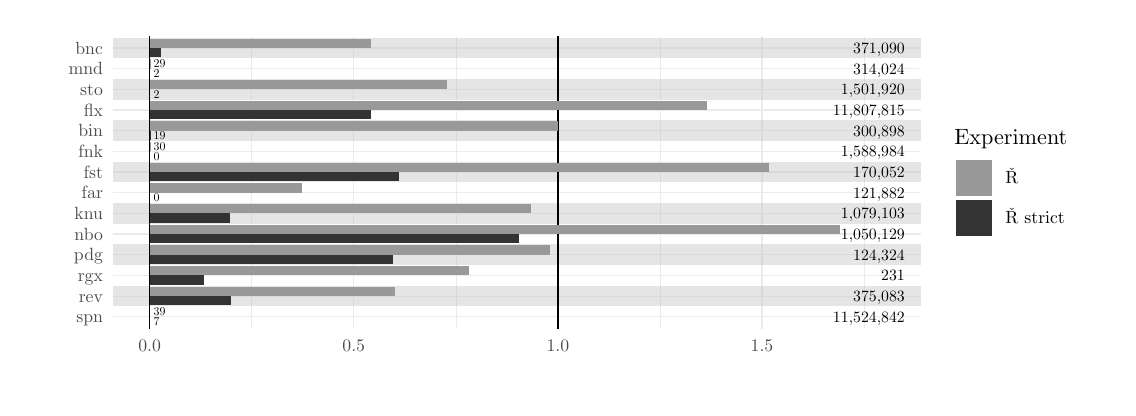
\begin{tikzpicture}[x=1pt,y=1pt]
\definecolor{fillColor}{RGB}{255,255,255}
\path[use as bounding box,fill=fillColor,fill opacity=0.00] (0,0) rectangle (390.26,130.09);
\begin{scope}
\path[clip] ( 30.80, 21.16) rectangle (322.87,127.24);
\definecolor{drawColor}{gray}{0.92}

\path[draw=drawColor,line width= 0.2pt,line join=round] ( 80.95, 21.16) --
	( 80.95,127.24);

\path[draw=drawColor,line width= 0.2pt,line join=round] (154.71, 21.16) --
	(154.71,127.24);

\path[draw=drawColor,line width= 0.2pt,line join=round] (228.46, 21.16) --
	(228.46,127.24);

\path[draw=drawColor,line width= 0.2pt,line join=round] (302.21, 21.16) --
	(302.21,127.24);

\path[draw=drawColor,line width= 0.4pt,line join=round] ( 30.80, 25.64) --
	(322.87, 25.64);

\path[draw=drawColor,line width= 0.4pt,line join=round] ( 30.80, 33.11) --
	(322.87, 33.11);

\path[draw=drawColor,line width= 0.4pt,line join=round] ( 30.80, 40.59) --
	(322.87, 40.59);

\path[draw=drawColor,line width= 0.4pt,line join=round] ( 30.80, 48.06) --
	(322.87, 48.06);

\path[draw=drawColor,line width= 0.4pt,line join=round] ( 30.80, 55.53) --
	(322.87, 55.53);

\path[draw=drawColor,line width= 0.4pt,line join=round] ( 30.80, 63.00) --
	(322.87, 63.00);

\path[draw=drawColor,line width= 0.4pt,line join=round] ( 30.80, 70.47) --
	(322.87, 70.47);

\path[draw=drawColor,line width= 0.4pt,line join=round] ( 30.80, 77.94) --
	(322.87, 77.94);

\path[draw=drawColor,line width= 0.4pt,line join=round] ( 30.80, 85.41) --
	(322.87, 85.41);

\path[draw=drawColor,line width= 0.4pt,line join=round] ( 30.80, 92.88) --
	(322.87, 92.88);

\path[draw=drawColor,line width= 0.4pt,line join=round] ( 30.80,100.35) --
	(322.87,100.35);

\path[draw=drawColor,line width= 0.4pt,line join=round] ( 30.80,107.82) --
	(322.87,107.82);

\path[draw=drawColor,line width= 0.4pt,line join=round] ( 30.80,115.29) --
	(322.87,115.29);

\path[draw=drawColor,line width= 0.4pt,line join=round] ( 30.80,122.76) --
	(322.87,122.76);

\path[draw=drawColor,line width= 0.4pt,line join=round] ( 44.07, 21.16) --
	( 44.07,127.24);

\path[draw=drawColor,line width= 0.4pt,line join=round] (117.83, 21.16) --
	(117.83,127.24);

\path[draw=drawColor,line width= 0.4pt,line join=round] (191.58, 21.16) --
	(191.58,127.24);

\path[draw=drawColor,line width= 0.4pt,line join=round] (265.34, 21.16) --
	(265.34,127.24);
\definecolor{fillColor}{RGB}{190,190,190}

\path[fill=fillColor,fill opacity=0.40] ( 30.80, 29.38) rectangle (322.87, 36.85);

\path[fill=fillColor,fill opacity=0.40] ( 30.80, 44.32) rectangle (322.87, 51.79);

\path[fill=fillColor,fill opacity=0.40] ( 30.80, 59.26) rectangle (322.87, 66.73);

\path[fill=fillColor,fill opacity=0.40] ( 30.80, 74.20) rectangle (322.87, 81.67);

\path[fill=fillColor,fill opacity=0.40] ( 30.80, 89.14) rectangle (322.87, 96.61);

\path[fill=fillColor,fill opacity=0.40] ( 30.80,104.08) rectangle (322.87,111.55);

\path[fill=fillColor,fill opacity=0.40] ( 30.80,119.02) rectangle (322.87,126.49);
\definecolor{drawColor}{RGB}{0,0,0}

\path[draw=drawColor,line width= 0.6pt,line join=round] (191.58, 21.16) -- (191.58,127.24);
\definecolor{fillColor}{gray}{0.20}

\path[fill=fillColor] ( 44.07,119.40) rectangle ( 48.25,122.76);

\path[fill=fillColor] ( 44.07,119.40) rectangle ( 48.25,122.76);

\path[fill=fillColor] ( 44.07,119.40) rectangle ( 48.25,122.76);

\path[fill=fillColor] ( 44.07,119.40) rectangle ( 48.25,122.76);

\path[fill=fillColor] ( 44.07,119.40) rectangle ( 48.25,122.76);

\path[fill=fillColor] ( 44.07,119.40) rectangle ( 48.25,122.76);

\path[fill=fillColor] ( 44.07,119.40) rectangle ( 48.25,122.76);

\path[fill=fillColor] ( 44.07,119.40) rectangle ( 48.25,122.76);

\path[fill=fillColor] ( 44.07,119.40) rectangle ( 48.25,122.76);

\path[fill=fillColor] ( 44.07,119.40) rectangle ( 48.25,122.76);
\definecolor{fillColor}{gray}{0.60}

\path[fill=fillColor] ( 44.07,122.76) rectangle (124.16,126.12);

\path[fill=fillColor] ( 44.07,122.76) rectangle (124.16,126.12);

\path[fill=fillColor] ( 44.07,122.76) rectangle (124.16,126.12);

\path[fill=fillColor] ( 44.07,122.76) rectangle (124.16,126.12);

\path[fill=fillColor] ( 44.07,122.76) rectangle (124.16,126.12);

\path[fill=fillColor] ( 44.07,122.76) rectangle (124.16,126.12);

\path[fill=fillColor] ( 44.07,122.76) rectangle (124.16,126.12);

\path[fill=fillColor] ( 44.07,122.76) rectangle (124.16,126.12);

\path[fill=fillColor] ( 44.07,122.76) rectangle (124.16,126.12);

\path[fill=fillColor] ( 44.07,122.76) rectangle (124.16,126.12);
\definecolor{fillColor}{gray}{0.20}

\path[fill=fillColor] ( 44.07,111.93) rectangle ( 44.07,115.29);

\path[fill=fillColor] ( 44.07,111.93) rectangle ( 44.07,115.29);

\path[fill=fillColor] ( 44.07,111.93) rectangle ( 44.07,115.29);

\path[fill=fillColor] ( 44.07,111.93) rectangle ( 44.07,115.29);

\path[fill=fillColor] ( 44.07,111.93) rectangle ( 44.07,115.29);

\path[fill=fillColor] ( 44.07,111.93) rectangle ( 44.07,115.29);

\path[fill=fillColor] ( 44.07,111.93) rectangle ( 44.07,115.29);

\path[fill=fillColor] ( 44.07,111.93) rectangle ( 44.07,115.29);

\path[fill=fillColor] ( 44.07,111.93) rectangle ( 44.07,115.29);

\path[fill=fillColor] ( 44.07,111.93) rectangle ( 44.07,115.29);
\definecolor{fillColor}{gray}{0.60}

\path[fill=fillColor] ( 44.07,115.29) rectangle ( 44.09,118.65);

\path[fill=fillColor] ( 44.07,115.29) rectangle ( 44.09,118.65);

\path[fill=fillColor] ( 44.07,115.29) rectangle ( 44.09,118.65);

\path[fill=fillColor] ( 44.07,115.29) rectangle ( 44.09,118.65);

\path[fill=fillColor] ( 44.07,115.29) rectangle ( 44.09,118.65);

\path[fill=fillColor] ( 44.07,115.29) rectangle ( 44.09,118.65);

\path[fill=fillColor] ( 44.07,115.29) rectangle ( 44.09,118.65);

\path[fill=fillColor] ( 44.07,115.29) rectangle ( 44.09,118.65);

\path[fill=fillColor] ( 44.07,115.29) rectangle ( 44.09,118.65);

\path[fill=fillColor] ( 44.07,115.29) rectangle ( 44.09,118.65);
\definecolor{fillColor}{gray}{0.20}

\path[fill=fillColor] ( 44.07,104.46) rectangle ( 44.07,107.82);

\path[fill=fillColor] ( 44.07,104.46) rectangle ( 44.07,107.82);

\path[fill=fillColor] ( 44.07,104.46) rectangle ( 44.07,107.82);

\path[fill=fillColor] ( 44.07,104.46) rectangle ( 44.07,107.82);

\path[fill=fillColor] ( 44.07,104.46) rectangle ( 44.07,107.82);

\path[fill=fillColor] ( 44.07,104.46) rectangle ( 44.07,107.82);

\path[fill=fillColor] ( 44.07,104.46) rectangle ( 44.07,107.82);

\path[fill=fillColor] ( 44.07,104.46) rectangle ( 44.07,107.82);

\path[fill=fillColor] ( 44.07,104.46) rectangle ( 44.07,107.82);

\path[fill=fillColor] ( 44.07,104.46) rectangle ( 44.07,107.82);
\definecolor{fillColor}{gray}{0.60}

\path[fill=fillColor] ( 44.07,107.82) rectangle (151.35,111.18);

\path[fill=fillColor] ( 44.07,107.82) rectangle (151.35,111.18);

\path[fill=fillColor] ( 44.07,107.82) rectangle (151.35,111.18);

\path[fill=fillColor] ( 44.07,107.82) rectangle (151.35,111.18);

\path[fill=fillColor] ( 44.07,107.82) rectangle (151.35,111.18);

\path[fill=fillColor] ( 44.07,107.82) rectangle (151.35,111.18);

\path[fill=fillColor] ( 44.07,107.82) rectangle (151.35,111.18);

\path[fill=fillColor] ( 44.07,107.82) rectangle (151.35,111.18);

\path[fill=fillColor] ( 44.07,107.82) rectangle (151.35,111.18);

\path[fill=fillColor] ( 44.07,107.82) rectangle (151.35,111.18);
\definecolor{fillColor}{gray}{0.20}

\path[fill=fillColor] ( 44.07, 96.99) rectangle (124.05,100.35);

\path[fill=fillColor] ( 44.07, 96.99) rectangle (124.05,100.35);

\path[fill=fillColor] ( 44.07, 96.99) rectangle (124.05,100.35);

\path[fill=fillColor] ( 44.07, 96.99) rectangle (124.05,100.35);

\path[fill=fillColor] ( 44.07, 96.99) rectangle (124.05,100.35);

\path[fill=fillColor] ( 44.07, 96.99) rectangle (124.05,100.35);

\path[fill=fillColor] ( 44.07, 96.99) rectangle (124.05,100.35);

\path[fill=fillColor] ( 44.07, 96.99) rectangle (124.05,100.35);

\path[fill=fillColor] ( 44.07, 96.99) rectangle (124.05,100.35);

\path[fill=fillColor] ( 44.07, 96.99) rectangle (124.05,100.35);
\definecolor{fillColor}{gray}{0.60}

\path[fill=fillColor] ( 44.07,100.35) rectangle (245.34,103.71);

\path[fill=fillColor] ( 44.07,100.35) rectangle (245.34,103.71);

\path[fill=fillColor] ( 44.07,100.35) rectangle (245.34,103.71);

\path[fill=fillColor] ( 44.07,100.35) rectangle (245.34,103.71);

\path[fill=fillColor] ( 44.07,100.35) rectangle (245.34,103.71);

\path[fill=fillColor] ( 44.07,100.35) rectangle (245.34,103.71);

\path[fill=fillColor] ( 44.07,100.35) rectangle (245.34,103.71);

\path[fill=fillColor] ( 44.07,100.35) rectangle (245.34,103.71);

\path[fill=fillColor] ( 44.07,100.35) rectangle (245.34,103.71);

\path[fill=fillColor] ( 44.07,100.35) rectangle (245.34,103.71);
\definecolor{fillColor}{gray}{0.20}

\path[fill=fillColor] ( 44.07, 89.52) rectangle ( 44.08, 92.88);

\path[fill=fillColor] ( 44.07, 89.52) rectangle ( 44.08, 92.88);

\path[fill=fillColor] ( 44.07, 89.52) rectangle ( 44.08, 92.88);

\path[fill=fillColor] ( 44.07, 89.52) rectangle ( 44.08, 92.88);

\path[fill=fillColor] ( 44.07, 89.52) rectangle ( 44.08, 92.88);

\path[fill=fillColor] ( 44.07, 89.52) rectangle ( 44.08, 92.88);

\path[fill=fillColor] ( 44.07, 89.52) rectangle ( 44.08, 92.88);

\path[fill=fillColor] ( 44.07, 89.52) rectangle ( 44.08, 92.88);

\path[fill=fillColor] ( 44.07, 89.52) rectangle ( 44.08, 92.88);

\path[fill=fillColor] ( 44.07, 89.52) rectangle ( 44.08, 92.88);
\definecolor{fillColor}{gray}{0.60}

\path[fill=fillColor] ( 44.07, 92.88) rectangle (191.57, 96.24);

\path[fill=fillColor] ( 44.07, 92.88) rectangle (191.57, 96.24);

\path[fill=fillColor] ( 44.07, 92.88) rectangle (191.57, 96.24);

\path[fill=fillColor] ( 44.07, 92.88) rectangle (191.57, 96.24);

\path[fill=fillColor] ( 44.07, 92.88) rectangle (191.57, 96.24);

\path[fill=fillColor] ( 44.07, 92.88) rectangle (191.57, 96.24);

\path[fill=fillColor] ( 44.07, 92.88) rectangle (191.57, 96.24);

\path[fill=fillColor] ( 44.07, 92.88) rectangle (191.57, 96.24);

\path[fill=fillColor] ( 44.07, 92.88) rectangle (191.57, 96.24);

\path[fill=fillColor] ( 44.07, 92.88) rectangle (191.57, 96.24);
\definecolor{fillColor}{gray}{0.20}

\path[fill=fillColor] ( 44.07, 82.05) rectangle ( 44.07, 85.41);

\path[fill=fillColor] ( 44.07, 82.05) rectangle ( 44.07, 85.41);

\path[fill=fillColor] ( 44.07, 82.05) rectangle ( 44.07, 85.41);

\path[fill=fillColor] ( 44.07, 82.05) rectangle ( 44.07, 85.41);

\path[fill=fillColor] ( 44.07, 82.05) rectangle ( 44.07, 85.41);

\path[fill=fillColor] ( 44.07, 82.05) rectangle ( 44.07, 85.41);

\path[fill=fillColor] ( 44.07, 82.05) rectangle ( 44.07, 85.41);

\path[fill=fillColor] ( 44.07, 82.05) rectangle ( 44.07, 85.41);

\path[fill=fillColor] ( 44.07, 82.05) rectangle ( 44.07, 85.41);

\path[fill=fillColor] ( 44.07, 82.05) rectangle ( 44.07, 85.41);
\definecolor{fillColor}{gray}{0.60}

\path[fill=fillColor] ( 44.07, 85.41) rectangle ( 44.08, 88.77);

\path[fill=fillColor] ( 44.07, 85.41) rectangle ( 44.08, 88.77);

\path[fill=fillColor] ( 44.07, 85.41) rectangle ( 44.08, 88.77);

\path[fill=fillColor] ( 44.07, 85.41) rectangle ( 44.08, 88.77);

\path[fill=fillColor] ( 44.07, 85.41) rectangle ( 44.08, 88.77);

\path[fill=fillColor] ( 44.07, 85.41) rectangle ( 44.08, 88.77);

\path[fill=fillColor] ( 44.07, 85.41) rectangle ( 44.08, 88.77);

\path[fill=fillColor] ( 44.07, 85.41) rectangle ( 44.08, 88.77);

\path[fill=fillColor] ( 44.07, 85.41) rectangle ( 44.08, 88.77);

\path[fill=fillColor] ( 44.07, 85.41) rectangle ( 44.08, 88.77);
\definecolor{fillColor}{gray}{0.20}

\path[fill=fillColor] ( 44.07, 74.57) rectangle (134.29, 77.94);

\path[fill=fillColor] ( 44.07, 74.57) rectangle (134.29, 77.94);

\path[fill=fillColor] ( 44.07, 74.57) rectangle (134.29, 77.94);

\path[fill=fillColor] ( 44.07, 74.57) rectangle (134.29, 77.94);

\path[fill=fillColor] ( 44.07, 74.57) rectangle (134.29, 77.94);

\path[fill=fillColor] ( 44.07, 74.57) rectangle (134.29, 77.94);

\path[fill=fillColor] ( 44.07, 74.57) rectangle (134.29, 77.94);

\path[fill=fillColor] ( 44.07, 74.57) rectangle (134.29, 77.94);

\path[fill=fillColor] ( 44.07, 74.57) rectangle (134.29, 77.94);

\path[fill=fillColor] ( 44.07, 74.57) rectangle (134.29, 77.94);
\definecolor{fillColor}{gray}{0.60}

\path[fill=fillColor] ( 44.07, 77.94) rectangle (267.90, 81.30);

\path[fill=fillColor] ( 44.07, 77.94) rectangle (267.90, 81.30);

\path[fill=fillColor] ( 44.07, 77.94) rectangle (267.90, 81.30);

\path[fill=fillColor] ( 44.07, 77.94) rectangle (267.90, 81.30);

\path[fill=fillColor] ( 44.07, 77.94) rectangle (267.90, 81.30);

\path[fill=fillColor] ( 44.07, 77.94) rectangle (267.90, 81.30);

\path[fill=fillColor] ( 44.07, 77.94) rectangle (267.90, 81.30);

\path[fill=fillColor] ( 44.07, 77.94) rectangle (267.90, 81.30);

\path[fill=fillColor] ( 44.07, 77.94) rectangle (267.90, 81.30);

\path[fill=fillColor] ( 44.07, 77.94) rectangle (267.90, 81.30);
\definecolor{fillColor}{gray}{0.20}

\path[fill=fillColor] ( 44.07, 67.10) rectangle ( 44.07, 70.47);

\path[fill=fillColor] ( 44.07, 67.10) rectangle ( 44.07, 70.47);

\path[fill=fillColor] ( 44.07, 67.10) rectangle ( 44.07, 70.47);

\path[fill=fillColor] ( 44.07, 67.10) rectangle ( 44.07, 70.47);

\path[fill=fillColor] ( 44.07, 67.10) rectangle ( 44.07, 70.47);

\path[fill=fillColor] ( 44.07, 67.10) rectangle ( 44.07, 70.47);

\path[fill=fillColor] ( 44.07, 67.10) rectangle ( 44.07, 70.47);

\path[fill=fillColor] ( 44.07, 67.10) rectangle ( 44.07, 70.47);

\path[fill=fillColor] ( 44.07, 67.10) rectangle ( 44.07, 70.47);

\path[fill=fillColor] ( 44.07, 67.10) rectangle ( 44.07, 70.47);
\definecolor{fillColor}{gray}{0.60}

\path[fill=fillColor] ( 44.07, 70.47) rectangle ( 98.96, 73.83);

\path[fill=fillColor] ( 44.07, 70.47) rectangle ( 98.96, 73.83);

\path[fill=fillColor] ( 44.07, 70.47) rectangle ( 98.96, 73.83);

\path[fill=fillColor] ( 44.07, 70.47) rectangle ( 98.96, 73.83);

\path[fill=fillColor] ( 44.07, 70.47) rectangle ( 98.96, 73.83);

\path[fill=fillColor] ( 44.07, 70.47) rectangle ( 98.96, 73.83);

\path[fill=fillColor] ( 44.07, 70.47) rectangle ( 98.96, 73.83);

\path[fill=fillColor] ( 44.07, 70.47) rectangle ( 98.96, 73.83);

\path[fill=fillColor] ( 44.07, 70.47) rectangle ( 98.96, 73.83);

\path[fill=fillColor] ( 44.07, 70.47) rectangle ( 98.96, 73.83);
\definecolor{fillColor}{gray}{0.20}

\path[fill=fillColor] ( 44.07, 59.63) rectangle ( 73.24, 63.00);

\path[fill=fillColor] ( 44.07, 59.63) rectangle ( 73.24, 63.00);

\path[fill=fillColor] ( 44.07, 59.63) rectangle ( 73.24, 63.00);

\path[fill=fillColor] ( 44.07, 59.63) rectangle ( 73.24, 63.00);

\path[fill=fillColor] ( 44.07, 59.63) rectangle ( 73.24, 63.00);

\path[fill=fillColor] ( 44.07, 59.63) rectangle ( 73.24, 63.00);

\path[fill=fillColor] ( 44.07, 59.63) rectangle ( 73.24, 63.00);

\path[fill=fillColor] ( 44.07, 59.63) rectangle ( 73.24, 63.00);

\path[fill=fillColor] ( 44.07, 59.63) rectangle ( 73.24, 63.00);

\path[fill=fillColor] ( 44.07, 59.63) rectangle ( 73.24, 63.00);
\definecolor{fillColor}{gray}{0.60}

\path[fill=fillColor] ( 44.07, 63.00) rectangle (181.99, 66.36);

\path[fill=fillColor] ( 44.07, 63.00) rectangle (181.99, 66.36);

\path[fill=fillColor] ( 44.07, 63.00) rectangle (181.99, 66.36);

\path[fill=fillColor] ( 44.07, 63.00) rectangle (181.99, 66.36);

\path[fill=fillColor] ( 44.07, 63.00) rectangle (181.99, 66.36);

\path[fill=fillColor] ( 44.07, 63.00) rectangle (181.99, 66.36);

\path[fill=fillColor] ( 44.07, 63.00) rectangle (181.99, 66.36);

\path[fill=fillColor] ( 44.07, 63.00) rectangle (181.99, 66.36);

\path[fill=fillColor] ( 44.07, 63.00) rectangle (181.99, 66.36);

\path[fill=fillColor] ( 44.07, 63.00) rectangle (181.99, 66.36);
\definecolor{fillColor}{gray}{0.20}

\path[fill=fillColor] ( 44.07, 52.16) rectangle (177.53, 55.53);

\path[fill=fillColor] ( 44.07, 52.16) rectangle (177.53, 55.53);

\path[fill=fillColor] ( 44.07, 52.16) rectangle (177.53, 55.53);

\path[fill=fillColor] ( 44.07, 52.16) rectangle (177.53, 55.53);

\path[fill=fillColor] ( 44.07, 52.16) rectangle (177.53, 55.53);

\path[fill=fillColor] ( 44.07, 52.16) rectangle (177.53, 55.53);

\path[fill=fillColor] ( 44.07, 52.16) rectangle (177.53, 55.53);

\path[fill=fillColor] ( 44.07, 52.16) rectangle (177.53, 55.53);

\path[fill=fillColor] ( 44.07, 52.16) rectangle (177.53, 55.53);

\path[fill=fillColor] ( 44.07, 52.16) rectangle (177.53, 55.53);
\definecolor{fillColor}{gray}{0.60}

\path[fill=fillColor] ( 44.07, 55.53) rectangle (293.42, 58.89);

\path[fill=fillColor] ( 44.07, 55.53) rectangle (293.42, 58.89);

\path[fill=fillColor] ( 44.07, 55.53) rectangle (293.42, 58.89);

\path[fill=fillColor] ( 44.07, 55.53) rectangle (293.42, 58.89);

\path[fill=fillColor] ( 44.07, 55.53) rectangle (293.42, 58.89);

\path[fill=fillColor] ( 44.07, 55.53) rectangle (293.42, 58.89);

\path[fill=fillColor] ( 44.07, 55.53) rectangle (293.42, 58.89);

\path[fill=fillColor] ( 44.07, 55.53) rectangle (293.42, 58.89);

\path[fill=fillColor] ( 44.07, 55.53) rectangle (293.42, 58.89);

\path[fill=fillColor] ( 44.07, 55.53) rectangle (293.42, 58.89);
\definecolor{fillColor}{gray}{0.20}

\path[fill=fillColor] ( 44.07, 44.69) rectangle (132.13, 48.06);

\path[fill=fillColor] ( 44.07, 44.69) rectangle (132.13, 48.06);

\path[fill=fillColor] ( 44.07, 44.69) rectangle (132.13, 48.06);

\path[fill=fillColor] ( 44.07, 44.69) rectangle (132.13, 48.06);

\path[fill=fillColor] ( 44.07, 44.69) rectangle (132.13, 48.06);

\path[fill=fillColor] ( 44.07, 44.69) rectangle (132.13, 48.06);

\path[fill=fillColor] ( 44.07, 44.69) rectangle (132.13, 48.06);

\path[fill=fillColor] ( 44.07, 44.69) rectangle (132.13, 48.06);

\path[fill=fillColor] ( 44.07, 44.69) rectangle (132.13, 48.06);

\path[fill=fillColor] ( 44.07, 44.69) rectangle (132.13, 48.06);
\definecolor{fillColor}{gray}{0.60}

\path[fill=fillColor] ( 44.07, 48.06) rectangle (188.90, 51.42);

\path[fill=fillColor] ( 44.07, 48.06) rectangle (188.90, 51.42);

\path[fill=fillColor] ( 44.07, 48.06) rectangle (188.90, 51.42);

\path[fill=fillColor] ( 44.07, 48.06) rectangle (188.90, 51.42);

\path[fill=fillColor] ( 44.07, 48.06) rectangle (188.90, 51.42);

\path[fill=fillColor] ( 44.07, 48.06) rectangle (188.90, 51.42);

\path[fill=fillColor] ( 44.07, 48.06) rectangle (188.90, 51.42);

\path[fill=fillColor] ( 44.07, 48.06) rectangle (188.90, 51.42);

\path[fill=fillColor] ( 44.07, 48.06) rectangle (188.90, 51.42);

\path[fill=fillColor] ( 44.07, 48.06) rectangle (188.90, 51.42);
\definecolor{fillColor}{gray}{0.20}

\path[fill=fillColor] ( 44.07, 37.22) rectangle ( 63.87, 40.59);

\path[fill=fillColor] ( 44.07, 37.22) rectangle ( 63.87, 40.59);

\path[fill=fillColor] ( 44.07, 37.22) rectangle ( 63.87, 40.59);

\path[fill=fillColor] ( 44.07, 37.22) rectangle ( 63.87, 40.59);

\path[fill=fillColor] ( 44.07, 37.22) rectangle ( 63.87, 40.59);

\path[fill=fillColor] ( 44.07, 37.22) rectangle ( 63.87, 40.59);

\path[fill=fillColor] ( 44.07, 37.22) rectangle ( 63.87, 40.59);

\path[fill=fillColor] ( 44.07, 37.22) rectangle ( 63.87, 40.59);

\path[fill=fillColor] ( 44.07, 37.22) rectangle ( 63.87, 40.59);

\path[fill=fillColor] ( 44.07, 37.22) rectangle ( 63.87, 40.59);
\definecolor{fillColor}{gray}{0.60}

\path[fill=fillColor] ( 44.07, 40.59) rectangle (159.65, 43.95);

\path[fill=fillColor] ( 44.07, 40.59) rectangle (159.65, 43.95);

\path[fill=fillColor] ( 44.07, 40.59) rectangle (159.65, 43.95);

\path[fill=fillColor] ( 44.07, 40.59) rectangle (159.65, 43.95);

\path[fill=fillColor] ( 44.07, 40.59) rectangle (159.65, 43.95);

\path[fill=fillColor] ( 44.07, 40.59) rectangle (159.65, 43.95);

\path[fill=fillColor] ( 44.07, 40.59) rectangle (159.65, 43.95);

\path[fill=fillColor] ( 44.07, 40.59) rectangle (159.65, 43.95);

\path[fill=fillColor] ( 44.07, 40.59) rectangle (159.65, 43.95);

\path[fill=fillColor] ( 44.07, 40.59) rectangle (159.65, 43.95);
\definecolor{fillColor}{gray}{0.20}

\path[fill=fillColor] ( 44.07, 29.75) rectangle ( 73.57, 33.11);

\path[fill=fillColor] ( 44.07, 29.75) rectangle ( 73.57, 33.11);

\path[fill=fillColor] ( 44.07, 29.75) rectangle ( 73.57, 33.11);

\path[fill=fillColor] ( 44.07, 29.75) rectangle ( 73.57, 33.11);

\path[fill=fillColor] ( 44.07, 29.75) rectangle ( 73.57, 33.11);

\path[fill=fillColor] ( 44.07, 29.75) rectangle ( 73.57, 33.11);

\path[fill=fillColor] ( 44.07, 29.75) rectangle ( 73.57, 33.11);

\path[fill=fillColor] ( 44.07, 29.75) rectangle ( 73.57, 33.11);

\path[fill=fillColor] ( 44.07, 29.75) rectangle ( 73.57, 33.11);

\path[fill=fillColor] ( 44.07, 29.75) rectangle ( 73.57, 33.11);
\definecolor{fillColor}{gray}{0.60}

\path[fill=fillColor] ( 44.07, 33.11) rectangle (132.58, 36.48);

\path[fill=fillColor] ( 44.07, 33.11) rectangle (132.58, 36.48);

\path[fill=fillColor] ( 44.07, 33.11) rectangle (132.58, 36.48);

\path[fill=fillColor] ( 44.07, 33.11) rectangle (132.58, 36.48);

\path[fill=fillColor] ( 44.07, 33.11) rectangle (132.58, 36.48);

\path[fill=fillColor] ( 44.07, 33.11) rectangle (132.58, 36.48);

\path[fill=fillColor] ( 44.07, 33.11) rectangle (132.58, 36.48);

\path[fill=fillColor] ( 44.07, 33.11) rectangle (132.58, 36.48);

\path[fill=fillColor] ( 44.07, 33.11) rectangle (132.58, 36.48);

\path[fill=fillColor] ( 44.07, 33.11) rectangle (132.58, 36.48);
\definecolor{fillColor}{gray}{0.20}

\path[fill=fillColor] ( 44.07, 22.28) rectangle ( 44.07, 25.64);

\path[fill=fillColor] ( 44.07, 22.28) rectangle ( 44.07, 25.64);

\path[fill=fillColor] ( 44.07, 22.28) rectangle ( 44.07, 25.64);

\path[fill=fillColor] ( 44.07, 22.28) rectangle ( 44.07, 25.64);

\path[fill=fillColor] ( 44.07, 22.28) rectangle ( 44.07, 25.64);

\path[fill=fillColor] ( 44.07, 22.28) rectangle ( 44.07, 25.64);

\path[fill=fillColor] ( 44.07, 22.28) rectangle ( 44.07, 25.64);

\path[fill=fillColor] ( 44.07, 22.28) rectangle ( 44.07, 25.64);

\path[fill=fillColor] ( 44.07, 22.28) rectangle ( 44.07, 25.64);

\path[fill=fillColor] ( 44.07, 22.28) rectangle ( 44.07, 25.64);
\definecolor{fillColor}{gray}{0.60}

\path[fill=fillColor] ( 44.07, 25.64) rectangle ( 44.07, 29.01);

\path[fill=fillColor] ( 44.07, 25.64) rectangle ( 44.07, 29.01);

\path[fill=fillColor] ( 44.07, 25.64) rectangle ( 44.07, 29.01);

\path[fill=fillColor] ( 44.07, 25.64) rectangle ( 44.07, 29.01);

\path[fill=fillColor] ( 44.07, 25.64) rectangle ( 44.07, 29.01);

\path[fill=fillColor] ( 44.07, 25.64) rectangle ( 44.07, 29.01);

\path[fill=fillColor] ( 44.07, 25.64) rectangle ( 44.07, 29.01);

\path[fill=fillColor] ( 44.07, 25.64) rectangle ( 44.07, 29.01);

\path[fill=fillColor] ( 44.07, 25.64) rectangle ( 44.07, 29.01);

\path[fill=fillColor] ( 44.07, 25.64) rectangle ( 44.07, 29.01);

\path[draw=drawColor,line width= 0.6pt,line join=round] ( 44.07, 21.16) -- ( 44.07,127.24);

\node[text=drawColor,anchor=base east,inner sep=0pt, outer sep=0pt, scale=  0.57] at (316.97,120.80) {   371,090};

\node[text=drawColor,anchor=base east,inner sep=0pt, outer sep=0pt, scale=  0.57] at (316.97,113.33) {   314,024};

\node[text=drawColor,anchor=base east,inner sep=0pt, outer sep=0pt, scale=  0.57] at (316.97,105.86) { 1,501,920};

\node[text=drawColor,anchor=base east,inner sep=0pt, outer sep=0pt, scale=  0.57] at (316.97, 98.39) {11,807,815};

\node[text=drawColor,anchor=base east,inner sep=0pt, outer sep=0pt, scale=  0.57] at (316.97, 90.92) {   300,898};

\node[text=drawColor,anchor=base east,inner sep=0pt, outer sep=0pt, scale=  0.57] at (316.97, 83.45) { 1,588,984};

\node[text=drawColor,anchor=base east,inner sep=0pt, outer sep=0pt, scale=  0.57] at (316.97, 75.98) {   170,052};

\node[text=drawColor,anchor=base east,inner sep=0pt, outer sep=0pt, scale=  0.57] at (316.97, 68.51) {   121,882};

\node[text=drawColor,anchor=base east,inner sep=0pt, outer sep=0pt, scale=  0.57] at (316.97, 61.04) { 1,079,103};

\node[text=drawColor,anchor=base east,inner sep=0pt, outer sep=0pt, scale=  0.57] at (316.97, 53.57) { 1,050,129};

\node[text=drawColor,anchor=base east,inner sep=0pt, outer sep=0pt, scale=  0.57] at (316.97, 46.10) {   124,324};

\node[text=drawColor,anchor=base east,inner sep=0pt, outer sep=0pt, scale=  0.57] at (316.97, 38.63) {       231};

\node[text=drawColor,anchor=base east,inner sep=0pt, outer sep=0pt, scale=  0.57] at (316.97, 31.15) {   375,083};

\node[text=drawColor,anchor=base east,inner sep=0pt, outer sep=0pt, scale=  0.57] at (316.97, 23.68) {11,524,842};

\node[text=drawColor,anchor=base west,inner sep=0pt, outer sep=0pt, scale=  0.43] at ( 45.55,115.69) {  29};

\node[text=drawColor,anchor=base west,inner sep=0pt, outer sep=0pt, scale=  0.43] at ( 45.55, 85.80) {  30};

\node[text=drawColor,anchor=base west,inner sep=0pt, outer sep=0pt, scale=  0.43] at ( 45.55, 26.04) {  39};

\node[text=drawColor,anchor=base west,inner sep=0pt, outer sep=0pt, scale=  0.43] at ( 45.55,111.95) {   2};

\node[text=drawColor,anchor=base west,inner sep=0pt, outer sep=0pt, scale=  0.43] at ( 45.55,104.48) {   2};

\node[text=drawColor,anchor=base west,inner sep=0pt, outer sep=0pt, scale=  0.43] at ( 45.55, 89.54) {  19};

\node[text=drawColor,anchor=base west,inner sep=0pt, outer sep=0pt, scale=  0.43] at ( 45.55, 82.07) {   0};

\node[text=drawColor,anchor=base west,inner sep=0pt, outer sep=0pt, scale=  0.43] at ( 45.55, 67.13) {   0};

\node[text=drawColor,anchor=base west,inner sep=0pt, outer sep=0pt, scale=  0.43] at ( 45.55, 22.31) {   7};
\end{scope}
\begin{scope}
\path[clip] (  0.00,  0.00) rectangle (390.26,130.09);
\definecolor{drawColor}{gray}{0.30}

\node[text=drawColor,anchor=base east,inner sep=0pt, outer sep=0pt, scale=  0.64] at ( 27.20, 23.44) {spn};

\node[text=drawColor,anchor=base east,inner sep=0pt, outer sep=0pt, scale=  0.64] at ( 27.20, 30.91) {rev};

\node[text=drawColor,anchor=base east,inner sep=0pt, outer sep=0pt, scale=  0.64] at ( 27.20, 38.38) {rgx};

\node[text=drawColor,anchor=base east,inner sep=0pt, outer sep=0pt, scale=  0.64] at ( 27.20, 45.85) {pdg};

\node[text=drawColor,anchor=base east,inner sep=0pt, outer sep=0pt, scale=  0.64] at ( 27.20, 53.32) {nbo};

\node[text=drawColor,anchor=base east,inner sep=0pt, outer sep=0pt, scale=  0.64] at ( 27.20, 60.79) {knu};

\node[text=drawColor,anchor=base east,inner sep=0pt, outer sep=0pt, scale=  0.64] at ( 27.20, 68.26) {far};

\node[text=drawColor,anchor=base east,inner sep=0pt, outer sep=0pt, scale=  0.64] at ( 27.20, 75.73) {fst};

\node[text=drawColor,anchor=base east,inner sep=0pt, outer sep=0pt, scale=  0.64] at ( 27.20, 83.20) {fnk};

\node[text=drawColor,anchor=base east,inner sep=0pt, outer sep=0pt, scale=  0.64] at ( 27.20, 90.67) {bin};

\node[text=drawColor,anchor=base east,inner sep=0pt, outer sep=0pt, scale=  0.64] at ( 27.20, 98.14) {flx};

\node[text=drawColor,anchor=base east,inner sep=0pt, outer sep=0pt, scale=  0.64] at ( 27.20,105.61) {sto};

\node[text=drawColor,anchor=base east,inner sep=0pt, outer sep=0pt, scale=  0.64] at ( 27.20,113.08) {mnd};

\node[text=drawColor,anchor=base east,inner sep=0pt, outer sep=0pt, scale=  0.64] at ( 27.20,120.55) {bnc};
\end{scope}
\begin{scope}
\path[clip] (  0.00,  0.00) rectangle (390.26,130.09);
\definecolor{drawColor}{gray}{0.30}

\node[text=drawColor,anchor=base,inner sep=0pt, outer sep=0pt, scale=  0.64] at ( 44.07, 13.15) {0.0};

\node[text=drawColor,anchor=base,inner sep=0pt, outer sep=0pt, scale=  0.64] at (117.83, 13.15) {0.5};

\node[text=drawColor,anchor=base,inner sep=0pt, outer sep=0pt, scale=  0.64] at (191.58, 13.15) {1.0};

\node[text=drawColor,anchor=base,inner sep=0pt, outer sep=0pt, scale=  0.64] at (265.34, 13.15) {1.5};
\end{scope}
\begin{scope}
\path[clip] (  0.00,  0.00) rectangle (390.26,130.09);
\definecolor{drawColor}{RGB}{0,0,0}

\node[text=drawColor,anchor=base west,inner sep=0pt, outer sep=0pt, scale=  0.80] at (334.87, 87.90) {Experiment};
\end{scope}
\begin{scope}
\path[clip] (  0.00,  0.00) rectangle (390.26,130.09);
\definecolor{fillColor}{gray}{0.60}

\path[fill=fillColor] (335.58, 69.38) rectangle (348.61, 82.41);
\end{scope}
\begin{scope}
\path[clip] (  0.00,  0.00) rectangle (390.26,130.09);
\definecolor{fillColor}{gray}{0.20}

\path[fill=fillColor] (335.58, 54.93) rectangle (348.61, 67.96);
\end{scope}
\begin{scope}
\path[clip] (  0.00,  0.00) rectangle (390.26,130.09);
\definecolor{drawColor}{RGB}{0,0,0}

\node[text=drawColor,anchor=base west,inner sep=0pt, outer sep=0pt, scale=  0.64] at (353.32, 73.69) {\v{R}};
\end{scope}
\begin{scope}
\path[clip] (  0.00,  0.00) rectangle (390.26,130.09);
\definecolor{drawColor}{RGB}{0,0,0}

\node[text=drawColor,anchor=base west,inner sep=0pt, outer sep=0pt, scale=  0.64] at (353.32, 59.24) {\v{R} strict};
\end{scope}
\end{tikzpicture}

%   \caption{Promises allocated, normalized to GNU R. The right column shows GNU R's actual promises. If the bar is too small to display, we show the actual number of promises in the respective experiment.}
%   \label{fig:gc-pressure}
% \end{figure}




\end{document}
